\documentclass[11pt, a4paper]{article}
\usepackage[utf8]{inputenc}
\usepackage[ngerman]{babel}
\usepackage{graphicx}

\begin{document}

\tableofcontents
\thispagestyle{empty}
\newpage

\section{Einleitung}
Hier eine kurze Einleitung in welchem Rahmen diese Arbeit entstanden ist und schonmal ganz kurz auf SETI eingehen.

\section{SETI Breakthrough Listen}
Die kaggle Challenge \emph{SETI Breakthrough Listen - E.T. Signal Search} war ein öffentlicher Machine Learning Wettbewerb des \emph{Berkeley SETI Research Centers} im Zeitraum vom 10. Mai 2021 bis 18. August 2021. Die zugrunde liegenden Daten sind noch verfügbar, sodass Interessierte sich nach wie vor mit diesem Problem beschäftigen können. Im folgenden werden wir die Challenge stets abgekürzt als \emph{SETI} bezeichnen. 

Die Herausforderung bei \emph{SETI} besteht darin, Spektrogramme, also eine bildliche Darstellung eines Frequenzbereichs in einem bestimmten Zeitraum, die basierend auf Rohdaten des \emph{Green Bank Telescopes} generiert worden sind, auf das Vorkommen von künstlich hinzugefügten extraterrestrischen Signalen zu untersuchen. Hierbei ist es wichtig, diese Signale von irdisches Signalen, wie etwa einem Radiosignal, zu unterscheiden. Um diese Unterscheidung vornehmen zu können, sind jeweils sechs Spektrogramme zusammengefasst, wobei die Spektrogramme eins, drei und fünf jeweils Aufnahmen des zu untersuchenden Ziels \glqq A\grqq{} sind und die übrigen jeweils auf Aufnahmen eines anderen Himmelskörpers \glqq B\grqq{}, \glqq C\grqq{} und \glqq D\grqq{}. Eine solche Gruppe von Spektrogrammen (ABACAD) wird bei \emph{SETI} als \emph{Kadenz-Ausschnitt}, im folgenden nur noch \glqq Kadenz\grqq{}, bezeichnet. Jedes Spektrogramm zeigt den Frequenzbereich für einen Zeitraum von fünf Minuten, eine Kadenz stellt folglich einen Beobachtungszeitraum von 30 Minuten dar.

Abbildung \ref{fig:kadenz_pos_1} zeigt ein Beispiel für eine Kadenz mit einem extraterrestrischen Signal. Die drei Spektrogramme in der oberen Zeile sind \emph{on target}, auf diesen ist im Frequenzbereich, welcher durch die x-Achse repräsentiert ist, zwischen 150 und 200 ein Signal zu erkennen, welches auf den Spektrogrammen in der unteren Zeile, welche \emph{off target} sind, nicht zu sehen ist. Die grüne senkrechte Linie, die auf allen sechs Spektogrammen zu sehen ist, ist hingegen ein irdisches Signal. Offensichtlich muss ein Signal nicht auf jedem der drei \emph{on target} Spektrogrammen zu sehen sein, da ein Signal nicht zwingend über den gesamten zeitlichen Betrachtungsraum aktiv sein muss.

\begin{figure}[t]
\centering
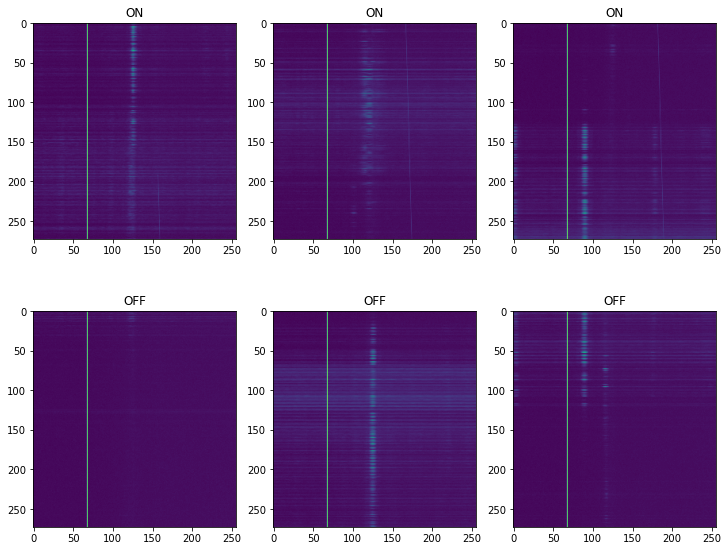
\includegraphics[width=0.9\textwidth]{"img/kadenz_pos_1.png"}
\caption{Beispiel für ein extraterrestrisches Signal}
\label{fig:kadenz_pos_1}
\end{figure}

Die Trainingsdaten für \emph{SETI} enthalten 60.000 Kadenzen (\emph{Heuhaufen}) von denen 6.000 \emph{Nadeln} sind, also Kadenzen, die ein künstlich eingefügtes extraterrestrisches Signal enthalten. Einige dieser Signale sind bei entsprechender Visualisierung sofort mit bloßem Auge zu erkennen, andere sind in, durch irdische Signale verursachten, Rauschen versteckt.


\section{Implementierung}
Im folgenden beschäftigen wir uns nun mit der Problemlösung für \emph{SETI}. Wir schauen uns erste Ansätze mit reiner Computer Vision an, die uns helfen sollen auch versteckte Signale extrahieren zu können, um sie mit bloßem Auge erkennen zu können. Wir haben uns für diesen Einstieg entschieden, um ein Gefühl für die visuelle Form der gesuchten Signale und für den Datensatz allgemein zu erhalten. Im darauf folgenden Kapitel werden wir uns mit \emph{Convulutional Neural Networks}, kurz \emph{CNNs}, beschäftigen.

\subsection{Erste Ansätze mit Computer Vision}
Hier können wir unseren ersten Ansätze mit reiner Computer Vision beschreiben und zunächst darauf eingehen, wie sich traditionelle Computer Vision von Machine Learning unterscheidet / abgrenzt und warum wir zunächst mit CV experimentiert haben.

\subsubsection{Implementierte CV Filter}
Hier können wir die Filter, die wir am Anfang implementiert haben jeweils kurz beschreiben

\subsubsection{Zwischenfazit: CV alleine bringt keinen Erfolg}
Kurzes Zwischenfazit, das CV alleine nichts nützt, weil die Signale selbst nach der Anwendung unserer Filter auf vielen Positives nicht zu extrahieren sind.

\section{Deep Learning}
Natürlich wollen wir nicht alle Kadenzen einzeln manuell betrachten und entscheiden, ob sie eine Nadel enthalten oder nicht. Vielmehr wollen wir ein Machine Learning Model trainieren, das uns diese Arbeit abnimmt und Nadeln findet, die wir gar nicht entdecken würden. Hierzu wollen wir ein \emph{Convolutional Neural Network (CNN)} trainieren, das die Kadenzen in genau zwei Klassen einteilt: enthält eine Nadel oder enthält keine Nadel.

\subsection{Convolutional Neural Networks}
Hier können wir uns nochmal überlegen oder mit Herrn Baier besprechen, wie doll wir bei den Erklärungen zu den einzelnen Punkten von CNNs ins Detail gehen sollen. Vll können wir auch vieles als bekannt voraussetzen und uns mehr auf unsere Implementierung konzentrieren. Dies wäre insgesamt vll nochmal abzuklären auch für die CV Section.

\begin{itemize}
	\item Gewichte
	\item Loss Function
	\item Gradient
	\item Optimizer
	\item Traning und Validierung
	\item Splitten der Trainingsdaten
	\item Dataloaders
	\item Metriken (Accuracy, Precision, Recall, F1 Score, Roc Auc Score)
\end{itemize}

\subsection{Transfer Learning}

\subsubsection{efficientnet}

\subsection{Imbalance}

\subsection{Scheduler}

\subsection{Folds}

\section{Tech Stack}
Zusammenfassung der verwendeten Tools und Bibliotheken, die teilweise auch vorher im Text schon genannt wurden.

\section{Fazit}


\end{document}